% Created 2014-11-08 Sat 11:30
\documentclass[presentation, bigger]{beamer}
\usepackage[utf8]{inputenc}
\usepackage[T1]{fontenc}
\usepackage{fixltx2e}
\usepackage{graphicx}
\usepackage{longtable}
\usepackage{float}
\usepackage{wrapfig}
\usepackage[normalem]{ulem}
\usepackage{textcomp}
\usepackage{marvosym}
\usepackage{wasysym}
\usepackage{latexsym}
\usepackage{amssymb}
\usepackage{amstext}
\usepackage{hyperref}
\usepackage{url}
\usepackage{multimedia}
\usepackage[dutch]{babel}
\usepackage[font=scriptsize,labelfont=bf]{caption}
\setbeamertemplate{caption}[numbered]
\usepackage{pgfpages}
\setbeameroption{show notes on second screen=right}

\tolerance=1000
\usetheme{kuleuven}
\useinnertheme{rectangles}
\graphicspath{{graphics/}}
\usepackage[style=authoryear,hyperref,backref,square,natbib,ibidtracker=false]{biblatex}
\bibliography{bibliography}

\usepackage{graphicx}
\usetheme{default}
\author{Ward Schodts, Xavier Goás Aguililla}
\date{maandag 10 november 2014}
\title{Internet of Things code deployment metrics}
\hypersetup{
  pdfkeywords={},
  pdfsubject={},
  pdfcreator={Emacs 24.3.1 (Org mode N/A)}}



\newcommand{\aheader}[2]{\action<#1-|alert@#1>{#2}}
% first argument: slide number to appear from, second argument: content of header 
\newcommand{\hiddencell}[2]{\action<#1->{#2}}
% first argument: slide number to appear from, second argument: content of cell

\begin{document}

\maketitle
\begin{frame}[noframenumbering]{Outline}
  \tableofcontents
\end{frame}

% \begin{itemize}
% \item TODO hier een afbeelding zoeken en aan de hand hiervan uitleggen!
% \item bestaan uit embedded computers, zgn. ‘motes’
%   TODO foto/video van motes
% \item uitgerust met low-power radioantennes en sensoren
% \end{itemize}


\section{Inleiding tot wireless sensor networks}
\label{sec-1}
\begin{frame}[label=sec-1-1]{Wireless sensor networks: wat zijn ze? (1)}

  \begin{figure}
    \fbox{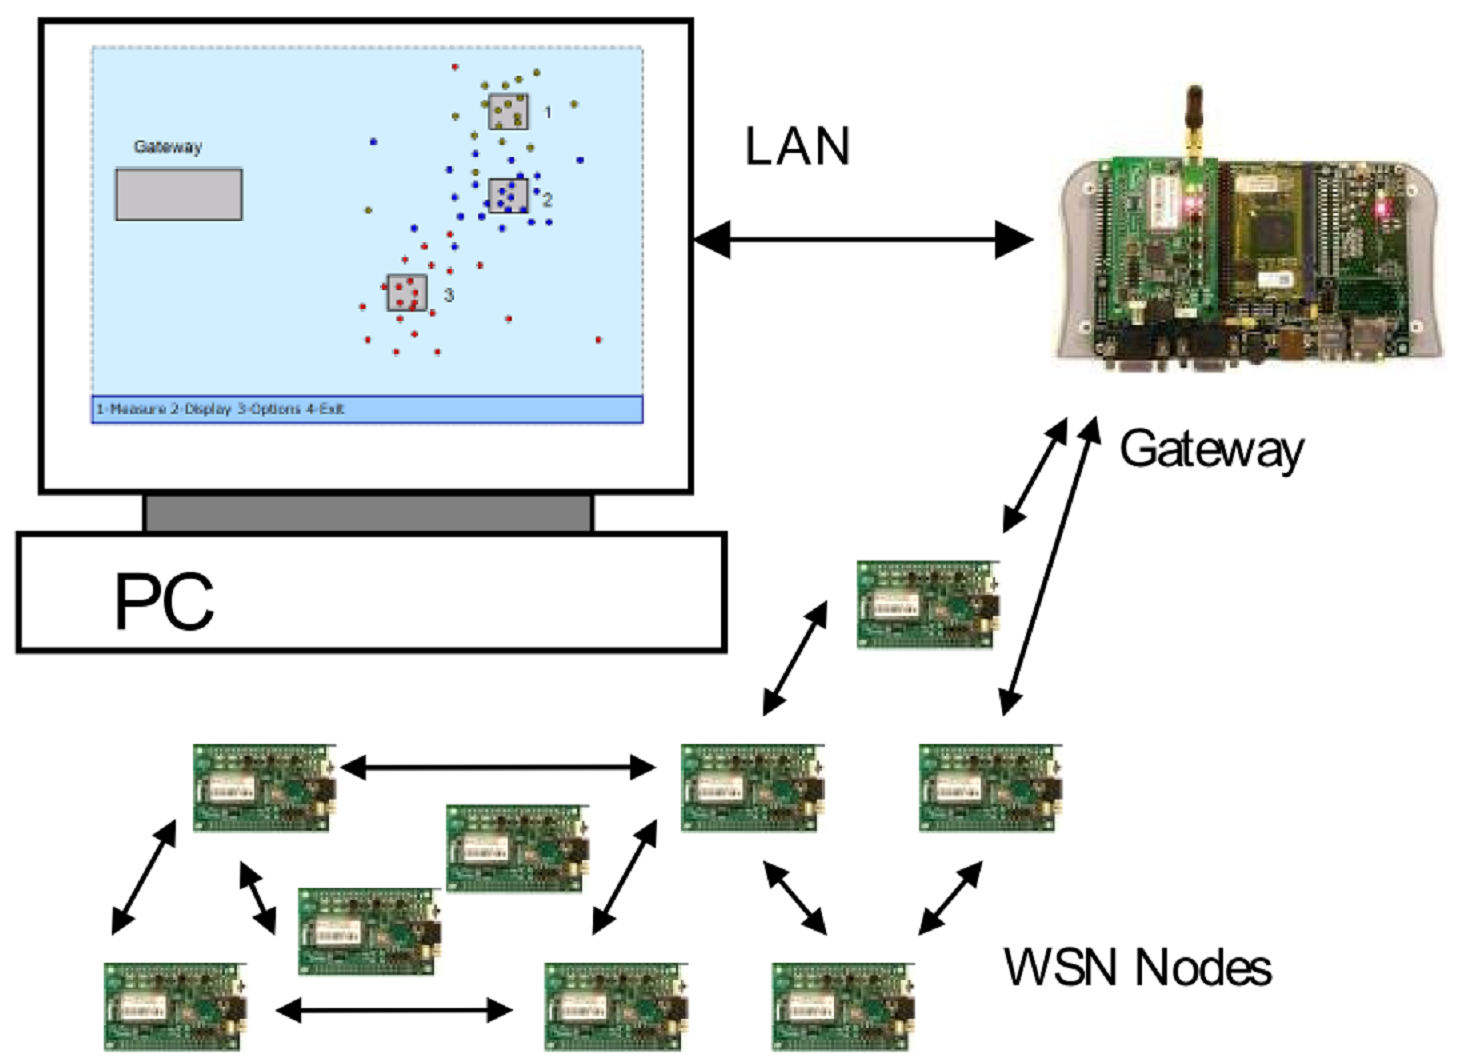
\includegraphics[width=0.82\textwidth,keepaspectration=true]{intro/overview.png}}
    \caption{Een wireless sensor network}
  \end{figure}

\end{frame}

\begin{frame}[label=sec-1-2]{Wireless sensor networks: wat zijn ze? (2)}
  \begin{figure}
    \fbox{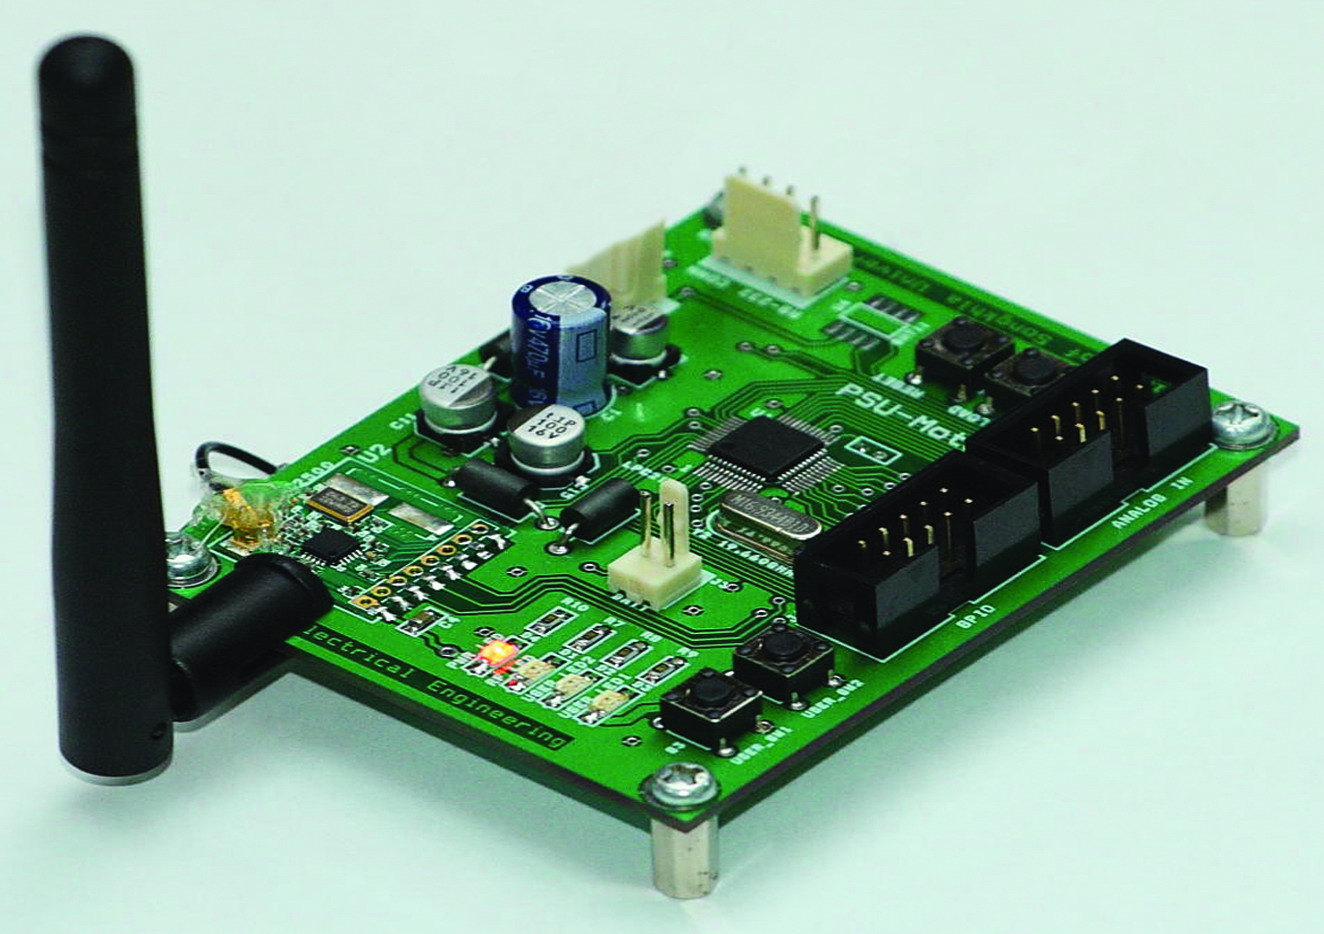
\includegraphics[height=0.78\textheight,keepaspectration=true]{intro/psumote.jpg}}
    \caption{Een PSUMote}
  \end{figure}

\end{frame}



\begin{frame}[label=sec-1-3]{Toepassingen van WSN}
  \centering 
  \begin{tabular}{c c c}
    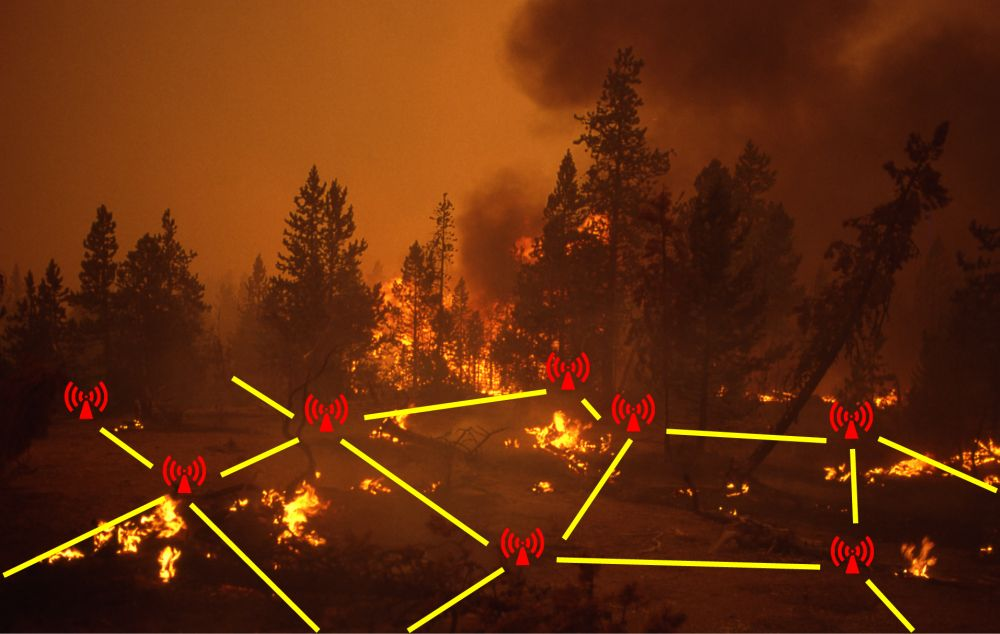
\includegraphics[width=5.25cm,keepaspectration=true]{graphics/sample_applications/fire.jpg}
    & 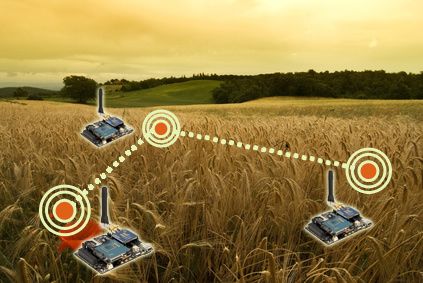
\includegraphics[width=5cm,keepaspectration=true]{graphics/sample_applications/landbouw.jpg} \\
    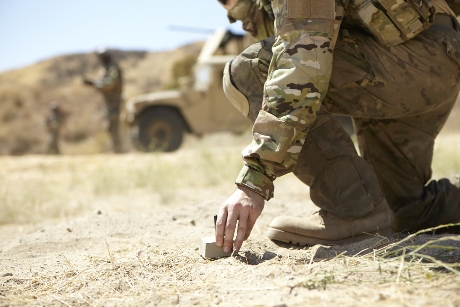
\includegraphics[width=5.25cm,keepaspectration=true]{graphics/sample_applications/military.jpg}
    & 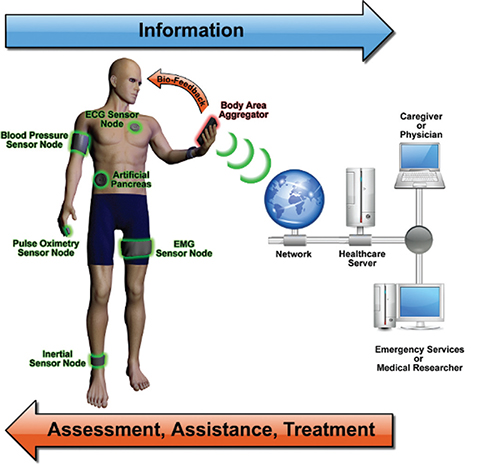
\includegraphics[width=5cm,keepaspectration=true]{graphics/sample_applications/medicine.jpg}
  \end{tabular}
  \note{and another test}

\end{frame}

\begin{frame}[label=sec-1-4]{Great Duck Island experiment I}
  \centering
  \begin{figure}
    \fbox{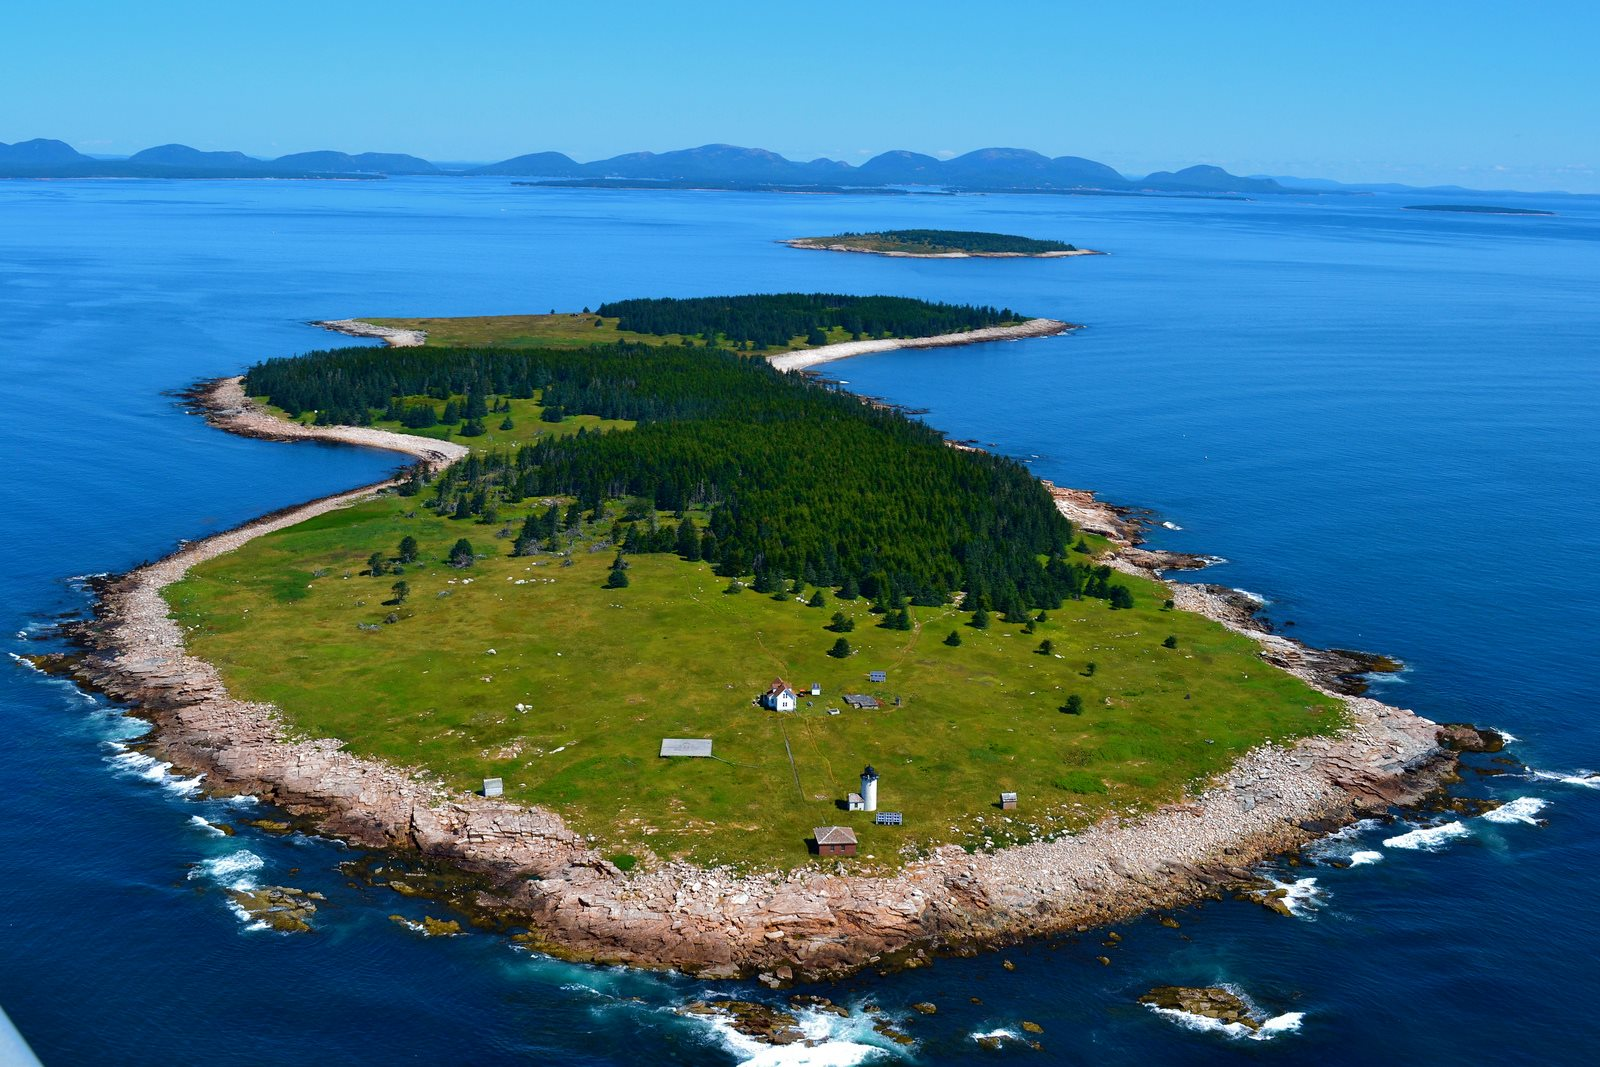
\includegraphics[width=0.85\textwidth,keepaspectratio=true]{gdi/gdi.jpg}}
    \caption{Great Duck Island}
  \end{figure}

\end{frame}
% TODO Beter woord voor monitoring vinden
\begin{frame}[label=sec-1-5]{Great Duck Island experiment II}
  \begin{figure}
    \begin{minipage}{.5\textwidth}
      \centering
      \fbox{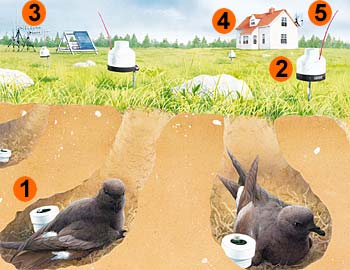
\includegraphics[width=.8\textwidth]{gdi/gdi_duckmote.jpg}} 
      \captionof{figure}{Motes in nesten}
    \end{minipage}%
    \begin{minipage}{.5\textwidth}
      \centering
      \fbox{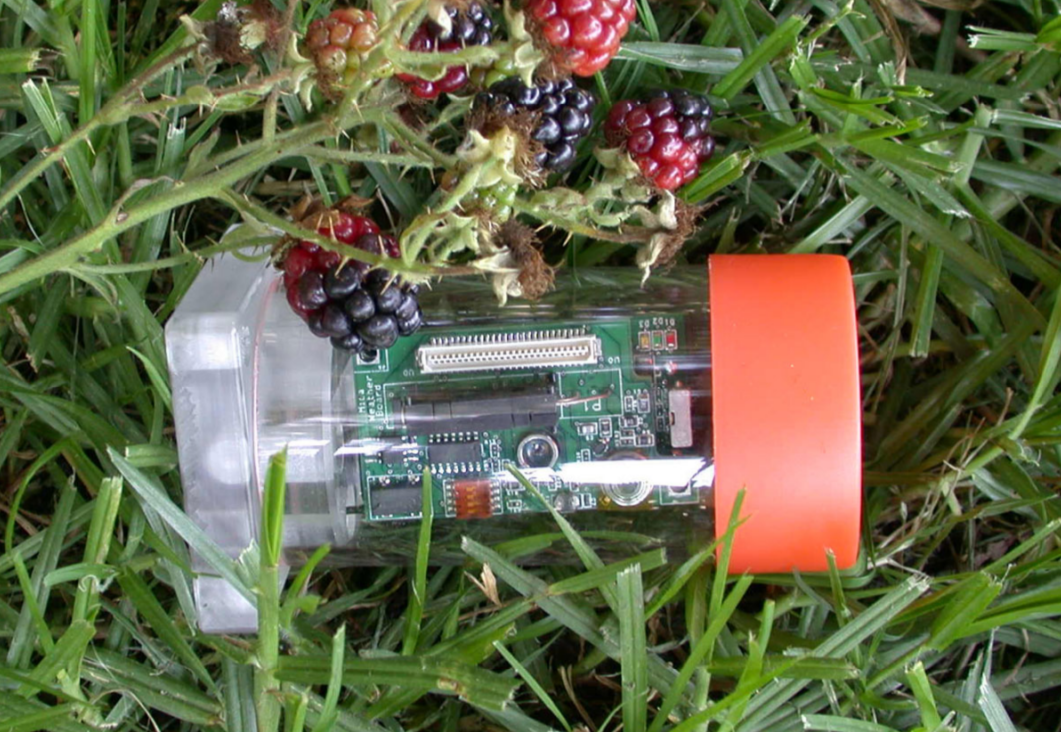
\includegraphics[width=.8\textwidth]{gdi/micamote.png}}
      \captionof{figure}{Motes in het gras}
    \end{minipage}
  \end{figure}
  \begin{itemize}
  \item habitat monitoring van eenden
  \item motes in broedholen
  \item 7 maanden
  \end{itemize}
  \note{
  \begin{itemize}
    \item Mensen konden niet in de buurt komen zonder te storen
    \item In de holen werden de motes gelegd
    \item En aanvullingen werden bijgezet
  \end{itemize}

  }
\end{frame}

\begin{frame}[label=sec-1-6]{Belangrijke aspecten bij WSN-design}
  \uncover<2->{\begin{block}{energie-effici\"ent}
      tot 10 jaar meegaan op \'e\'en batterij
    \end{block}}%
  \uncover<3->{\begin{block}{dichtheid}
      tot 20 sensor nodes per $m^3$ (geen harde limiet)
    \end{block}}%
  \uncover<4->{\begin{block}{goedkoop}
      \$1 of minder voor heel grootschalige deployments
    \end{block}}%
  \uncover<5->{\begin{block}{autonoom}
      deploy and forget
    \end{block}}%
  \uncover<6->{\begin{block}{adaptief}
      makkelijke aanpasbare topologie, bestand tegen falen van motes
    \end{block}}
  \note{Consume extremely low power, operate in high volumetric densities, have low production cost and be dispensable, be autonomous and operate unattended, be adaptive to the environment.}
\end{frame}

\section{Middleware voor WSNs}
\label{sec-2}
\begin{frame}[label=sec-2-1]{Wat is middleware?}
  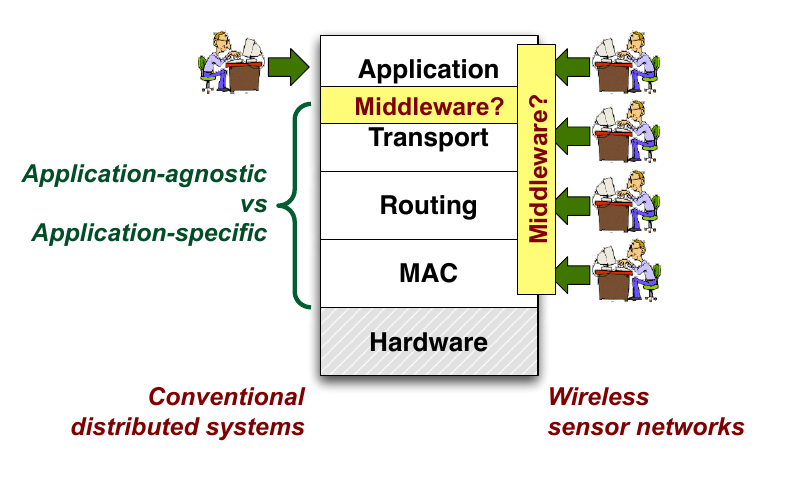
\includegraphics[width=\textwidth,keepaspectration=true]{middleware}
\end{frame}

\begin{frame}[label=sec-2-2]{Mogelijke aanpakken}
  \begin{itemize}
  \item application-based; bv. Contiki, Squawk
  \item component-based; bv. OpenCOM, Figaro, LooCi
    \begin{itemize}
    \item statisch
    \item dynamisch reconfigureerbaar
    \end{itemize}
  \end{itemize}
\end{frame}

\begin{frame}[label=sec-2-3]{LooCi (1)}
  \begin{columns}[t]
    \column{.5\textwidth}
    \centering
    
\includegraphics[width=5cm,keepaspectration=true]{looci/looci.png}\\
    
\includegraphics[width=5cm,keepaspectration=true]{looci/distrinet.png}
    \column{.5\textwidth}
    \centering
    \begin{itemize}
    \item Ontwikkeld aan KULeuven
    \item Runtime deployable components
    \item Werkt op Contiki, Sun SPOT, OSGi en Android
    \end{itemize}
  \end{columns}
\end{frame}

\begin{frame}[label=sec-2-4]{LooCi (2)}
  \centering
  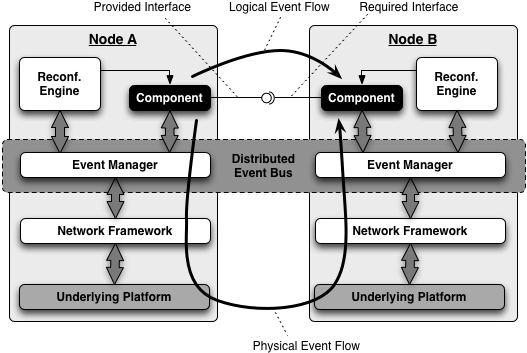
\includegraphics[width=0.9\textwidth,keepaspectration=true]{looci/LooCIExecEnvironment.png}
\end{frame}

\begin{frame}[label=sec-2-5]{LooCi demo}
  
\end{frame}

\section{Energieverbruik}
\label{sec-3}

\begin{frame}[label=sec-1-7]{Store, compute, transmit?}
  \begin{itemize}
  \item drie grote factoren in energieverbruik:
    \vfill
    \begin{tabular}{c c c}
      \hiddencell{2}{
\includegraphics[width=0.25\textwidth,keepaspectration=true]{storage}} & \hiddencell{3}{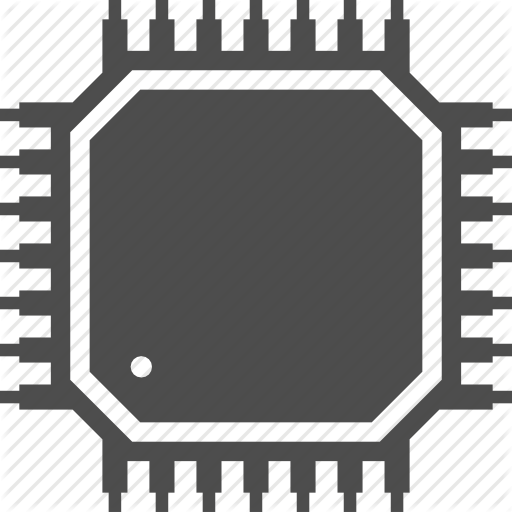
\includegraphics[width=0.25\textwidth,keepaspectration=true]{cpu}} & \hiddencell{4}{
\includegraphics[width=0.25\textwidth,keepaspectration=true]{radio}}  \\
      \hiddencell{2}{flash-opslag} & \hiddencell{3}{berekeningen} & \hiddencell{4}{netwerkoverdracht}
    \end{tabular}
    \vfill
  \item ook sensoren aangesloten op microcontroller hebben invloed
  \end{itemize}

    \note{
      \begin{itemize}
      \item antennes op en aan zetten kost veel energie
      \item flash en CPU iets minder, maar:
        \begin{itemize}
        \item lage kloksnelheid 
          \begin{itemize}
          \item slechte concurrency, 
          \item slechte performantie in het algemeen
          \end{itemize}
        \item beperkte hoeveelheid geheugen
        \end{itemize}
      \item huidige aanpak: veel netwerkoverdracht, weinig CPU- en geheugengebruik
      \end{itemize}
    }

\end{frame}


\begin{frame}[label=sec-3-2]{Hoe meten we het?}
  \begin{minipage}{\textwidth}
    \centering
    \fbox{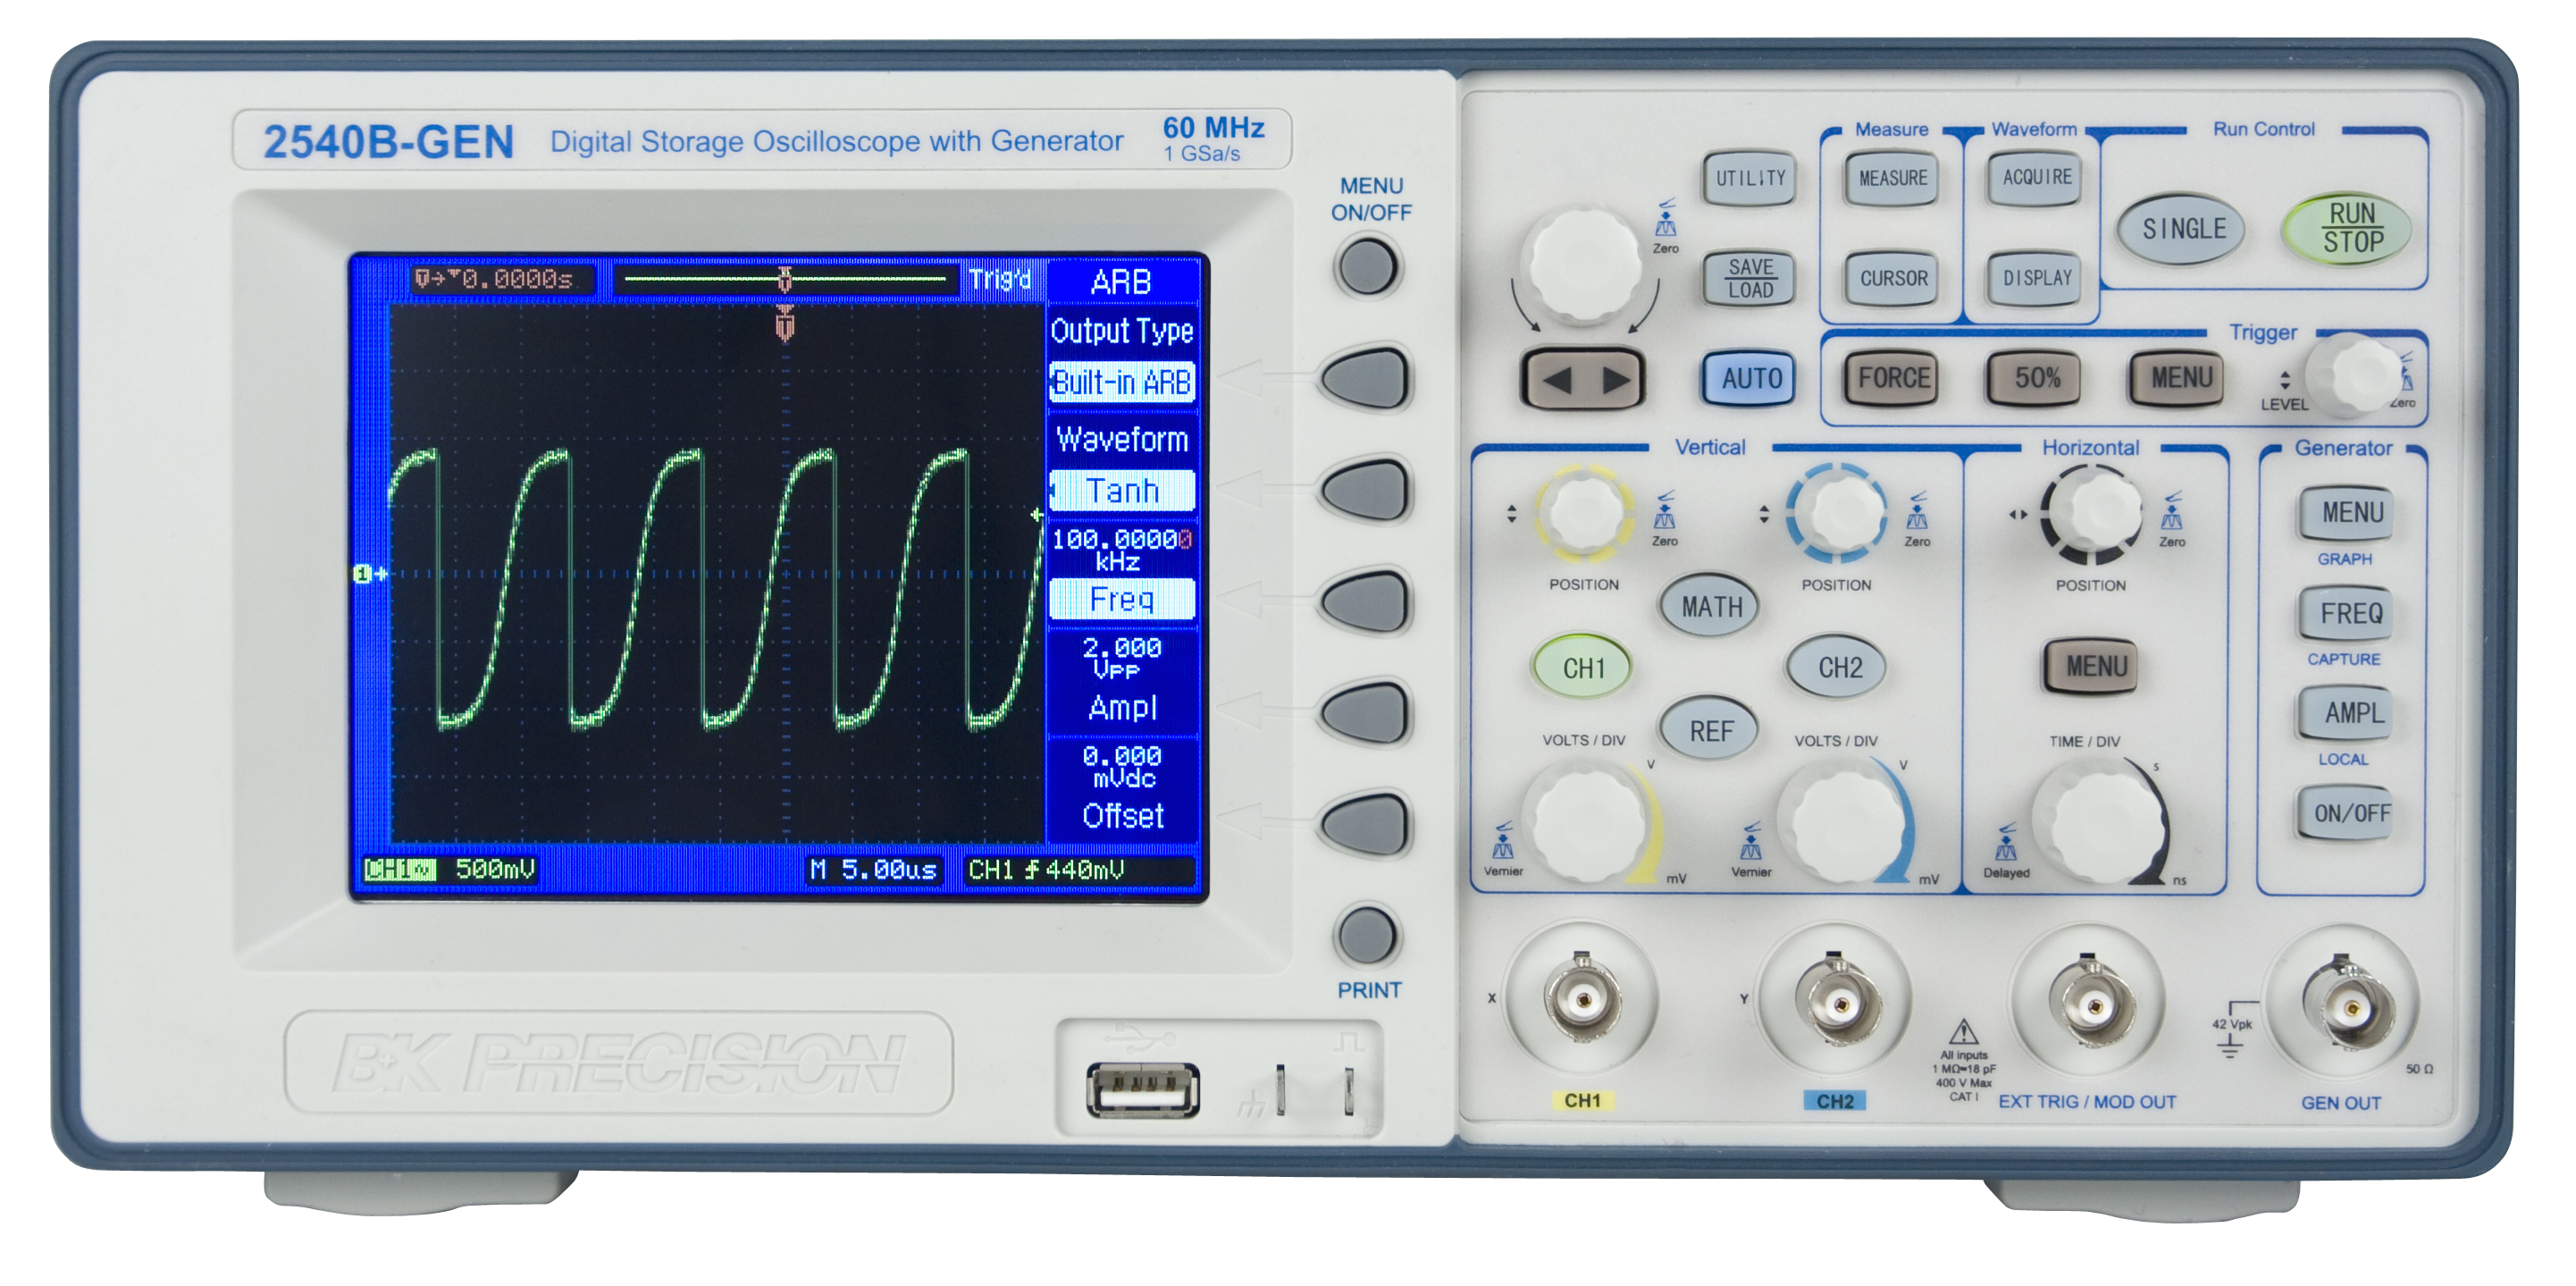
\includegraphics[width=0.9\textwidth,keepaspectration=true]{elek/dso.jpg}} 
    \captionof{figure}{Oscilloscoop}
  \end{minipage}

  \note{
    Oscilloscopes are used to observe the change of an electrical
signal over time, such that voltage and time describe a shape which is
continuously graphed against a calibrated scale.
    
    The observed waveform can be analyzed for such properties as
amplitude, frequency, rise time, time interval, distortion and others.
  }
\end{frame}

\begin{frame}[label=sec-3-3]{Meetopstelling}
  \begin{figure}[center]
    \centering
    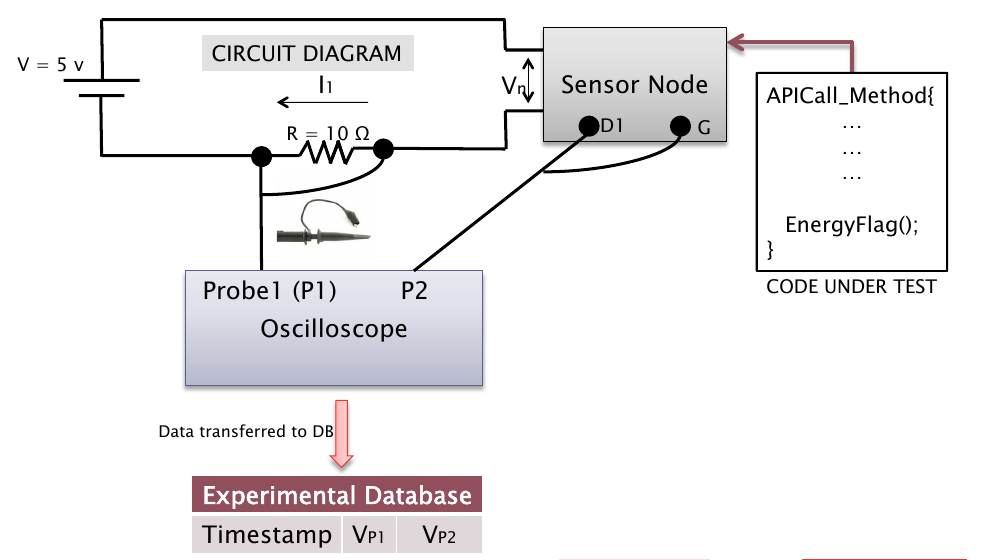
\includegraphics[width=0.9\textwidth,keepaspectration=true]{elek/diag1}
    \caption{Meetopstelling}
  \end{figure}
  \note{

    \begin{itemize}
    \item stroomverbruik van bepaalde methodes plotten
    \item opstelling: weerstand in serie geplaatst met stroomtoevoer
    \item oscilloscoop meet spanning
    \item start en stop mbv output pin
    \item outputpin softwarematig getriggerd
    \end{itemize}

Meetmethode:\\
\begin{itemize}
\item meerdere keren het te meten stuk code oproepen
\item pin zal verscheidene keren aan en uit flippen en metingen triggeren
\end{itemize}
  }
\end{frame}

\begin{frame}[label=sec-3-4]{Voltageplot}
  \begin{figure}
    \centering
    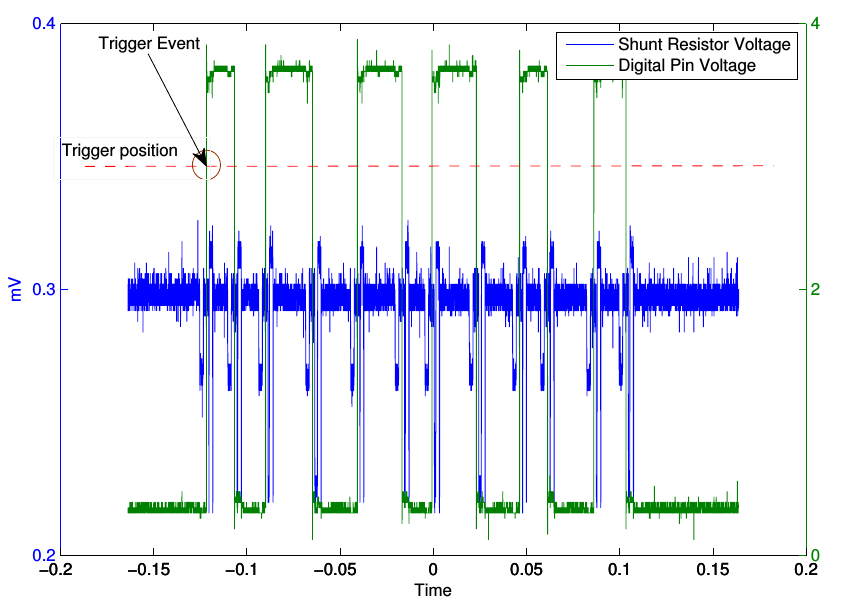
\includegraphics[width=0.85\textwidth,keepaspectration=true]{elek/energy_measurement_plot.png}
    \caption{Voltageplot}
  \end{figure}
  \note{
    Ziet er als volgt uit.

    \begin{itemize}
    \item blauw: voltage over weerstand
    \item groen: voltage op pin
    \end{itemize}
  }
\end{frame}

\begin{frame}[label=sec-3-5]{Analyse energieverbruik}
  \begin{itemize}
  \item wet van Ohm!
    \begin{figure}
      \centering
      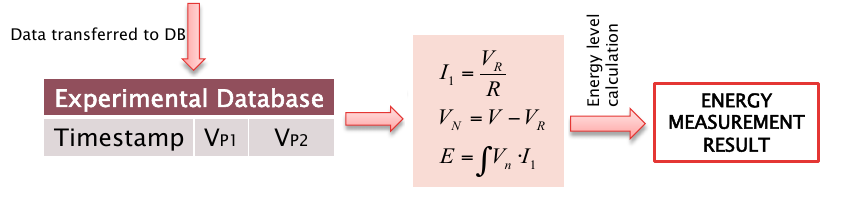
\includegraphics[width=0.9\textwidth,keepaspectration=true]{elek/diag2}

      \caption{Stroomverbruikanalyse}
    \end{figure}
  \item modelleren m.b.v. lineaire regressie
  \end{itemize}
  \note{

    \begin{itemize}
    \item gebruik de wet van Ohm
    \item accurate metingen van stroomverbruik van bepaalde methodes
    \item herhaal metingen tot we een goed idee hebben van \\ gemiddeld verbruik
    \end{itemize}

  }
\end{frame}
\section{Conclusie}
\label{sec-4}
\begin{frame}[label=sec-4-1]{Waar komen wij in het spel?}
  \begin{itemize}
  \item huidige aanpak in het veld: netwerk-overdracht
  \item is dit wel de enige goede methode?
  \item analyse stroomverbruik voor verschillende types code deployment
  \item implementeren tool voor simulatie energieverbruik
  \end{itemize}
\end{frame}

\begin{frame}[label=sec-4-2]{Conclusie}
  \begin{itemize}
  \item momenteel weinig aandacht voor alternatieve code deployment
  \item we hebben jullie een aantal idee\"en getoond 
  \item hier gaan we iets aan doen!
  \end{itemize}
\end{frame}
\begin{frame}[allowframebreaks]{Bibliografie}
  \nocite{*}
  \printbibliography
\end{frame}

% Emacs 24.3.1 (Org mode N/A)
\end{document}
